% Shared standalone design for the editable figure reconstructions.
\documentclass[tikz,border=5pt,10pt]{standalone}
\usepackage[T1]{fontenc}
\usepackage[utf8]{inputenc}
\usepackage{newpxtext,newpxmath}
\usepackage[scaled=.94]{sourcesanspro}
\usepackage{pgfplots}
\pgfplotsset{compat=1.18}
\usetikzlibrary{arrows.meta,calc,positioning,decorations.pathreplacing,
  decorations.markings,patterns,matrix,shapes.geometric,fit,backgrounds,
  intersections,angles,quotes}
\definecolor{ink}{HTML}{203746}
\definecolor{accent}{HTML}{146C78}
\definecolor{muted}{HTML}{667780}
\definecolor{signalred}{HTML}{B94B44}
\color{ink}
\tikzset{>=Latex,line width=.8pt,
  every node/.style={font=\small},
  axis/.style={->,draw=muted,line width=.5pt},
  guide/.style={draw=muted,dashed,line width=.45pt},
  curve/.style={draw=accent,line width=1pt},
  marker/.style={circle,fill=accent,inner sep=1.5pt},
  labelbox/.style={fill=white,inner sep=2pt}}

\begin{document}
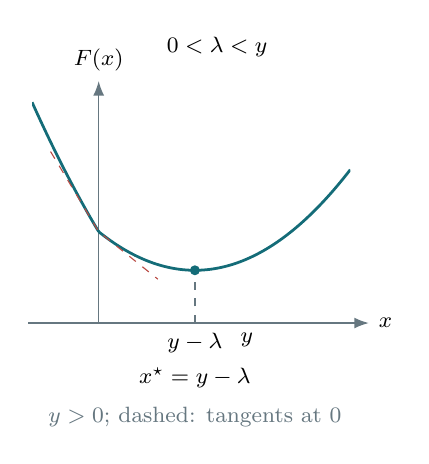
\begin{tikzpicture}[x=.94cm,y=.58cm,every node/.style={font=\footnotesize}]
\draw[axis] (-.95,0)--(3.65,0) node[right] {$x$};\draw[axis] (0,0)--(0,5.3) node[above] {$F(x)$};
\begin{scope}\clip (-.9,0) rectangle (3.4,5.1);
\draw[curve,domain=-.9:3.4,samples=180] plot (\x,{.5*(\x-2)^2+0.7*abs(\x)});
\draw[signalred,dashed] (-.65,{2+.65*(2+0.7)})--(0,2)--(.8,{2+.8*(0.7-2)});
\end{scope}
\draw[guide] (1.3,0)--(1.3,1.1549999999999998);\fill[accent] (1.3,1.1549999999999998) circle(1.8pt);
\node[below] at (2,0) {$y$};
\node[below] at (1.3,0) {$y-\lambda$};
\node at (1.6,6.05) {$0<\lambda<y$};
\node at (1.3,-1.2) {$x^\star=y-\lambda$};
\node[muted] at (1.3,-2.05) {$y>0$; dashed: tangents at $0$};
\end{tikzpicture}
\end{document}
